\documentclass{article} % use larger type; default would be 10pt

\usepackage[utf8]{inputenc} % set input encoding (not needed with XeLaTeX)

\usepackage{fixltx2e}
\usepackage{mdwlist}

%%% PAGE DIMENSIONS
\usepackage{geometry} % to change the page dimensions
\geometry{letterpaper} % or a4paper (Britain) or a5paper or....
% \geometry{margin=2in} % for example, change the margins to 2 inches all round
% \geometry{landscape} % set up the page for landscape
%   read geometry.pdf for detailed page layout information

\usepackage{graphicx} % support the \includegraphics command and options
\usepackage{xcolor}

%%% PACKAGES
\usepackage{booktabs} % for much better looking tables
\usepackage{array} % for better arrays (eg matrices) in maths
\usepackage{paralist} % very flexible & customisable lists (eg. enumerate/itemize, etc.)
\usepackage{verbatim} % adds environment for commenting out blocks of text & for better verbatim
\usepackage{subfig} % make it possible to include more than one captioned figure/table in a single float
\usepackage{amsmath}
\usepackage{pifont}
\usepackage[bottom]{footmisc}
\usepackage{setspace}

%%% HEADERS & FOOTERS
\usepackage{fancyhdr} % This should be set AFTER setting up the page geometry
\pagestyle{fancy} % options: empty , plain , fancy
\renewcommand{\headrulewidth}{0pt} % customise the layout...
\lhead{}\chead{}\rhead{}
\lfoot{}\cfoot{\thepage}\rfoot{}

%%% WIDOWS & ORPHANS
\widowpenalty=10000
\clubpenalty=10000

%%% SECTION TITLE APPEARANCE
\usepackage{sectsty}
\allsectionsfont{\sffamily\mdseries\upshape} % (See the fntguide.pdf for font help)

%%% ToC (table of contents) APPEARANCE
\usepackage[nottoc,notlof,notlot]{tocbibind} % Put the bibliography in the ToC
\usepackage[titles,subfigure]{tocloft} % Alter the style of the Table of Contents
\renewcommand{\cftsecfont}{\rmfamily\mdseries\upshape}
\renewcommand{\cftsecpagefont}{\rmfamily\mdseries\upshape} % No bold!

%%% END Article customizations


\title{Network of Networks\\Final Report}
\author{Hart Kornell\\ Special Technologies Lab\\National Security Technologies, LLC}
\date{30 September 2016} 


\begin{document}
\maketitle

\vfill
\begin{center}
US Department of Energy NNSA \\
\textbf{Defense Nuclear Nonproliferation R\&D} \\
WebPMIS: NST14-Network of Networks-PD3RS  \\
PI: J. Hart Kornell, NSTec, 805.452.8660, korneljm@nv.doe.gov \\
Co-PI: Zoe Gastelum, Sandia National Lab, 505.845.1002, zgastel@sandia.gov \\
Co-PI: Bethany L. Goldblum, UC Berkeley, bethany@nuc.berkeley.edu \\
HQ: James Peltz, 202.586.7564, james.peltz@nnsa.doe.gov \\
Funding start: 01 October 2013; Funding end: 30 September 2016
\end{center}
\newpage
\thispagestyle{empty}
\mbox{}
\newpage
\pagebreak
\hspace{0pt}
\vfill
\quote
The real purpose of the scientific method is to discover that nature hasn't misled you into thinking you know something you don't actually know. 

---Robert Pirsig, \textit{Zen and the Art of Motorcycle Maintenance}
\endquote
\vfill
\hspace{0pt}
\pagebreak

\newpage
\thispagestyle{empty}
\mbox{}
\newpage

\onehalfspace

\tableofcontents{}

\newpage
\thispagestyle{empty}
\mbox{}
\newpage

\section*{Network of Networks Summary}
\noindent Network of Networks was a program of  interdisciplinary research on modeling and analysis of complex networks in nonproliferation, proliferation detection, and safeguards. 

Substantial prior research in nonproliferation detection focused on detection of specific isotopes of elements of the periodic table. Since plain water can hide these, detection research expanded to include industrial-scale facilities associated with the nuclear fuel cycle, particularly with conversion and enrichment. 

In this research, we shifted assumptions to include the idea that inference over indirect evidence would be critical to complement the  direct sensing methods. We assumed the need to find patterns in incomplete, unreliable, time-sensitive, acyclic, sometimes-ambiguous,  sometimes-underdetermined, sometimes-intentionally-deceptive data. Our goal then became indicative patterns in complex networks. We built networks whose components were networks: networks of networks.

We have two chief findings:
\renewcommand\labelitemi{\tiny$\bullet$}
\begin{itemize*}
\item Different kinds of data can be integrated in multilayer, multiplex networks without distorting any individual network's internal structure or dynamics
\item The complex network approach can encompass and unify physical sensing, informational (`soft') sensing, and historical and context data.
\end{itemize*}

The work was performed by Hart Kornell of Special Technologies Laboratory (National Security Technologies, LLC), Zoe Gastelum of Sandia National Laboratories, and  Bethany L. Goldblum of the University of California at Berkeley, Nuclear Engineering Department. \textit{Acknowledgements} provides a more complete report of our indispensable contributors.

\newpage
\thispagestyle{empty}
\mbox{}
\newpage

\section{Introduction}
Nonproliferation and proliferation detection have changed over the decades as knowledge has spread. Not only application (`how-to') knowledge, but knowledge of how international monitoring, both open and covert, is performed. Since a well-organized proliferator or non-state actor knows both what's being looked for and to a significant extent how it's being looked for, new methods are needed.

Network science provides a relevant set of methods. If, as the authors believe, effective proliferation detection will require pattern discovery in combinations of physical evidence (from sensing), informational evidence (from open media), and the powerful constraints given by context, then network modeling and analysis is a viable approach to data integration.

We do not assert that networks are the only way to make progress. We do assert that they are \textit{a} way to make progress. \\

\begin{center}
\ding{118}
\end{center}

We document two streams in the work. 

First, we surveyed and assessed open media, including social media. `Open media' includes any information that is openly and freely available (including information behind a paywall, as with major newspapers.) Wikipedia, reports from the various Departments of the US government, the New York Times, and scientific publications are all examples of open media. `Social media' is a subset of open media, predominately focused on the ephemera of daily life.

Open media also includes historical data, which we used in the second research stream. There, we constructed a multiplex model of selected factors that can influence a nation's decision to proliferate. We limited our model to state-external factors. Our reasoning in making that cull was that because the method was new to this domain, the data informing the model should be as quantitatively uncontroversial as possible. We did not want subtly intrinsic features of the data to distort the focus on the utility of the method.

In the following pages we will (1) introduce multilayer and multiplex networks; (2) document our assessment of open and social media; and, (3) describe our historical model.

\newpage
\thispagestyle{empty}
\mbox{}
\newpage

\section{Networks, multilayer networks, and multiplex networks}
Networks are anything that can be made sense of by thinking of nodes and links.\footnote{Links are also called edges.} There are two features of this definition. First, networks are a mental construct. We frequently describe the world this way. For example, ecologists refer to a `wood wide web' when studying the anastomosis of tree roots and nutrient-transport fungi. The second feature follows the first, that how we construct networks depends on what we want to do with them. For a forester, the trees might be the nodes, while for a mycologist, the fungi are and the tress are the links. With networks as with most things, how we represent a problem depends on what we want to do to solve it.

Multilayer networks combine different networks or network fragments into a coherent whole. For instance, an urban multilayer network might include roads, electrical lines, water lines, and sewage systems as layers. Each of these might be a network on its own. In a multilayer network, the interactions and potential cascades that arise in the relationships between the layers can rigorously and repeatably characterize the behavior of the system as a whole.

Multiplex networks are a subset of multilayer networks, with the restriction that the nodes are shared among all network layers. For example, the reader may participate in a family network, a work network, and a friend network. Work and friend networks often have different dynamics than  family networks. This is a common example of a key power for multilayer and multiplex networks: each layer can have its own dynamics, its own way of working, its own characteristic timelines, and so on, independent of the other layers.

For nonproliferation and proliferation detection this is an elegant feature. If for example one component network is free within constraints and another is strictly deterministic, neither has to be distorted.  

\newpage
\thispagestyle{empty}
\mbox{}
\newpage

\section{Informational sensing: Traditional and new media}
We developed an overview of open source English-language data that can be used to support nuclear fuel cycle analysis, including both traditional open sources and `new media' sources. It also included some grey literature, i.e., information that is not completely open source such as data available to IAEA Safeguards staff members via internal databases. The document was intended to offer a preliminary understanding of some broad categories of information that may be available in open sources, and provide guidance on that data might be used to support fuel cycle analysis, including types of indicators potentially available in each source.

Traditional open sources referred to in the overview included both hard-copy and electronic sources of information that are (usually) publicly available, including news sources, scientific and technical literature, information on technical cooperation and education exchanges (referred to an internal-use IAEA database), trade and customs data, IAEA databases on declared nuclear capabilities, patent databases, nuclear trafficking data, individual government, university, and industry sites, and satellite and other imagery data. 

Social media refers to public content that is created by individuals for broader consumption, sharing, or viewing. Traditional social media is often limited in scope to platforms in which users define follow/friend/connection relationships with others to form a directed social network. New media is the high-volume, highly-interconnected, publicly available electronic (Internet) data produced by users who generate and publish data for open use. While this definition was at first limited to traditional social media sites in which users define mutual relationships with one another through shared interests or real-life connections, new media goes beyond the `known' social network to interactions facilitated via the internet of people, websites, and content. In new media, directed social relationship definitions are not required, and can include platforms such as social work sites, public blogs, comments on news sites, and so on. 

Social and new media sources included in the overview included blogs, microblogs (like Facebook and Instagram), social networking sites, photo, video, and audio sharing sites, wikis, social news, social games, geosocial apps, social elicitation (crowdsourcing), and review/recommendation sites. Social bookmarking, version control, and dark web sites were determined to be outside the scope of this overview.

An unclassified copy of the overview of traditional and new media is available upon request. Preliminary discussion of potential indicators is included only in a classified version of the overview.

Critical for the current work, incidental content may be found in social media that is relevant to nonproliferation or proliferation detection. Many amateur videos on YouTube and Vimeo sow nuclear material being transported. As well, information of interest shows up in the backgrounds of images that were not intended by their creator to capture nonproliferation-relevant data.

\subsection{S\&T Literature Analysis for Uranium Mining and Milling}
As the modeling effort focused on historical data, we considered how scientific and technical literature could be used to support the network  model described below. 

We collected 2,733 bibliographic records from the IAEA Nuclear Information Service database using a basic search string for uranium mining for the years 1948---1973.  From those records, we produced an index in the Sandia-developed software Citrus to aid  text analysis. We were able to determine the total number of times an author from one country published with someone from another country. 

This data drove multiple correlation experiments to determine if the number of a country's total publications related to uranium mining, their number of co-publications on uranium mining, or several normalized publication and co-publication metrics were related to the country's level of nuclear fuel cycle development, as represented in  Mathew Furhmann's nuclear capability database. We found that, for the publications and years that were included in our collection, the results were not significant. This result is interesting: it may mean that results of interest were entirely country-internal, that they were closely-held (classified) by the host government, or that the papers were biased toward basic physics and chemistry rather than applications. Regardless of cause, we consider it a useful result. 

\begin{tabular}{ |p{3.3cm}||p{2.5cm}|p{6cm}|  }
%\caption{Bibliographic records and uranium mining 1948---1973}
 \hline
 \multicolumn{3}{|c|}{\textbf{Publications and uranium mining}} \\
 \hline
 Experiment & Correlation & Notes\\
 \hline
 Co-publication to Capability   & 0.139851002    & This is the raw number\\
 \hline
 Country pubs to capability & 0.238236378  & Not normalized; we believe it results from general capability rising over time, as the number of country pubs also grew, due to digitization and growth in the field. \\
 \hline
 Normalized country pubs by INIS records/year to capability & -0.038097859 & Same as above, but normalizing country pub over total INIS records/year.\\
 \hline
 Normalized Copubs/country pubs to capability  & -0.151165955 & Normalizing copubs as a percentage of overall country pubs in a year\\
 \hline
 Normalized copubs/INIS records to capability &   -0.060949246 & Normalized copubs to total INIS records/year to account for growing body of INIS collection
\\
 \hline
\end{tabular}

Graph visualizations of the data by year are shown in the figure. The limited co-publication rate during the period under analysis made  such analysis non-definitive.

\begin{figure}
  \centering
  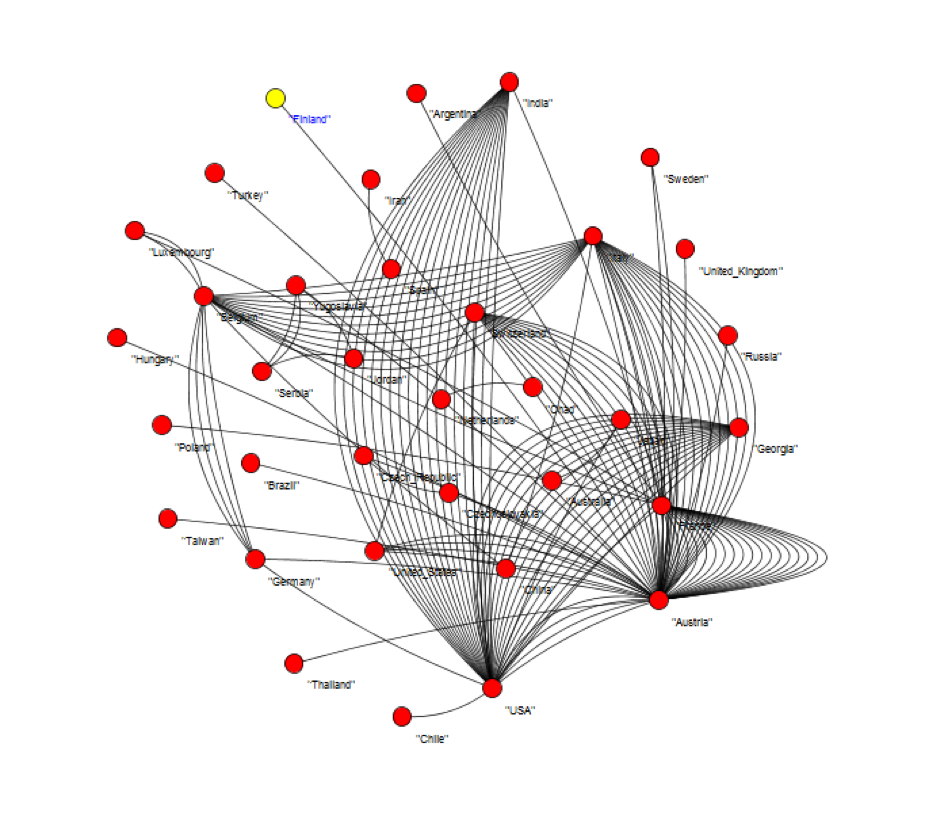
\includegraphics{all-country-year-co-pubs-uranium-mining48-73.png}
  \caption{Graph of all of the countries in the analysis, cumulative between 1948 and 1973.}
  \label{fig:allcountry4873}
\end{figure}

\newpage
\thispagestyle{empty}
\mbox{}
\newpage

\section{Model construction}
Determining which states will seek nuclear weapons has proven difficult for political scientists and policymakers. The nonproliferation community has long recognized the need to improve techniques for identifying state intent to acquire nuclear weapons (Fuhrmann 2009, 181--184; Fuhrmann and Sechser 2014, 461--463; Jo and Gartzke 2007; Montgomery and Sagan 2009, 302; Singh and Way 2004, 881--883). In response to this need, a significant body of international relations research has gone into determining which factors incentivize states to proliferate, focused on two main types of proliferation-relevant variables. First, several factors {\textit{internal}} to states have been identified as important, such as domestic politics, desire for prestige, and leadership psychology (Sagan 1996; Hymans 2010, 169--171). Second, several {\textit{external} factors have been identified, including armed conflicts, military alliances, international trade, and the transfer of nuclear technology and knowledge (Fuhrmann 2009; Jo and Gartzke 2007; Singh and Way 2004, 882). 

Political scientists have previously used network metrics such as symmetry, transitivity, and centrality to study international relations (Maoz 2009). This work examines the impact of external factors on proliferation likelihood using a new network-based formalism. Using open-source data, a multiplex network model was developed in which the sovereign states of the world (nodes) are connected through four relationship types (edges) thought to be {\textit{external}} determinants of nuclear proliferation: threat, alliances, nuclear cooperation agreements (NCAs), and trade. Using this approach, the structure of relational incentives and disincentives to proliferation are investigated, allowing for the potential extraction of otherwise subtle proliferation indicators. 

This model uses historical data to quantify each state's structural proliferation motivation as a node-based metric of its relations to other states. The structural proliferation metric (SPM) allows for an annual ranking of states from highest expectation of proliferation to lowest based on external determinants alone; an absolute proliferation likelihood is not provided, and internal determinants are beyond the scope of the study. Rankings of the SPM are then compared to the historical record for model validation and range of applicability. The SPM provides insight on the degree to which external factors alone can characterize a state's desire to produce nuclear weapons. Thus, the SPM may be used to gauge state proliferation interest by utilizing real-time, observable data on political and economic interactions, even in the absence of information on occurrences within state borders.

This subject matter was chosen for two reasons. First, using quantifications of aspects requiring human judgement shone a light on a topic often dismissed or avoided in nonproliferation, namely that any value assignment to an observation requires human judgement. In the nonproliferation community we often borrow the language and attitudes of lab scientists who are able experimentally to clamp all variables but for the one of interest, then rely on community consensus (as distilled in libraries) to judge whether the spectra collected match a canonical example. Human judgement is present at every step of that quantification chain. Similarly with our data, but more obviously. Second, our expectation was that the approach wouldn't work with regard to the subject matter. That is, we didn't the external factors alone would be close at all to observed behavior, believing as we did at the start that internal factors were central. We expected to quantify the inadequacies of an `external factor only' approach. We were surprised it worked as well as it did.


\subsection{Network Structure and Input}

\begin{figure}
\begin{center}
\includegraphics[scale=0.36]{layers.eps}
\caption{A multiplex network of proliferation-relevant international relations, with layers from top to bottom showing the NCA, alliance, threat, and trade relationships between nodes. Panel A shows a schematic network representation, where the nodes represent countries in the world. These nodes participate in all network layers, but the relationships between nodes (edges) are unique in each layer based on the relevant international relations. Panel B shows the full network representation of our model for the year 1980, built using open-source data.} 
\label{layers}
\end{center} 
\end{figure}

States are modeled as nodes in a network with consensus data from the literature used to quantify edges between the nodes representative of international relations. Nodes represent unitary states only; while non-state nuclear proliferation is an increasing threat to international security, the compilation of input data on international relations obtained from historical record precludes the consideration of non-state actors. As illustrated in Figure~\ref{layers}, each of the four international relationships\textemdash NCAs, alliances, threat, and trade\textemdash form a layer in the multiplex network. The edges are built on historical data from the period 1950--1992, where the date range examined in this study is based on data availability. Following Barrat, \textit{et al.}, edge weights are assigned in proportion to the intensity of the connections in the different network layers (Barrat et al. 2004). Each individual layer in the multiplex network can be disabled or enabled while other layers are held constant.

While factors such as armed conflict and alliances can be difficult to quantify, the literature provides consensus around several datasets that code these historical events and relationships in directed-dyad form. Where possible, datasets with a history of use in studies of nuclear proliferation are used. Data sources are summarized in Table~\ref{data}. The impact of the international relationships as relevant to nuclear proliferation are quantified using node-based metrics described in the following sections.

\begin{table}
\centering
\caption{Data Sources \label{data}}
\begin{tabular}{l@{\hskip 0.2in}p{0.55\linewidth}}
\hline\noalign{\smallskip}
Variable & Source(s) \\
\noalign{\smallskip}
\hline
\noalign{\smallskip}
Conventional Military Strength ($M$) & Correlates of War Composite Index of National Capability (Singer et al. 1972) \\
Nuclear Capability ($C$) & International Atomic Energy Agency (IAEA) Nuclear Fuel Cycle Information System (IAEA 2015a) \\ 
& IAEA Research Reactor Database (IAEA 2015b) \\
& Global Nuclear Weapons Inventory (Kristensen and Norris 2013) \\
 & World Nuclear Association (WNA) Reactor Database (WNA 2015)\\
Conflict Intensity ($I$) & Militarized Interstate Dispute Database (Jones et al. 1996) \\
Alliance Commitments ($a$) & Alliance and Treaty Obligation Project (ATOP) (Leeds et al. 2002) \\
Nuclear Cooperation Agreements ($n$) & NCA Database (Fuhrmann 2009) \\
Trade Dependence ($D$) & Triangulating Peace Replication Data (Russett and Oneal 2001) \\
\hline
\end{tabular}
\end{table}

\subsection{Threat}

Conflicts represent security threats that may influence states to explore, pursue, and acquire nuclear weapons (Jo and Gartzke 2007, 173--174; Singh and Way 2004, 882--883; Sagan 1996, 57--63). Edges in the single-layer threat network indicate the presence of a conflict between two states and are used to quantify a threat metric for each dyad. The security threat posed by a conflict is assumed to be modulated by the military capabilities of the adversary. That is, the threat perception posed by a conflict increases with increasing military capabilities of the adversary. The military strength, $S_i$, of node $i$ is given by the product of the conventional military strength, $M_i$, and nuclear capability, $C_i$, of node $i$:
\begin{center}
\begin{equation}
S_i = M_i C_i.
\end{equation}
\end{center}
Conventional military strength, $M$, is quantified using a Composite Index of National Capability score from the Correlates of War project (Singer et al. 1972). Nuclear capability, $C$, is quantified as shown in Table~\ref{tab:cap}. 

\begin{table}
\centering
\caption{Ranking of Nuclear Capability ($C$)
\label{tab:cap}}
\begin{tabular}{c@{\hskip 0.35in}l}
\hline\noalign{\smallskip}
Coding & Description\\
\noalign{\smallskip}
\hline
\noalign{\smallskip}
1 & No capability \\
2 & Laboratory-scale nuclear facilities \\
3 & Nuclear research reactor facilities \\
4 & Civilian nuclear power generation \\
5 & Enrichment and reprocessing \\
6 & Possession of nuclear device \\
\hline
\end{tabular} 
\end{table}

The measure of threat is a function of both conflict intensity, $I$, and balance of military strength, $S_{rel}$. The relative military strength, $S_{rel}$, is a pairwise comparison of the military strength of node $i$ relative to node $j$:
\begin{center}
\begin{equation}
\begin{aligned}
S_{rel}(ij) = \dfrac {S_i} {S_i + S_j}.
\end{aligned}
\end{equation}
\end{center}
Note that relative strength is an inverse relationship; as state $i$ increases in strength compared to state $j$, state $j$ grows correspondingly weaker than state $i$.

\begin{table}
\centering
\caption{Ranking of Conflict Intensity ($I$)
\label{tab:intensity}}
\begin{tabular}{c@{\hskip 0.25in}l}
\hline\noalign{\smallskip}
Coding & Description\\
\noalign{\smallskip}
\hline
\noalign{\smallskip}
1 & Recipient of conflict action (codes 2-4); does not respond \\
2  & Threat of force \\
3 & Display of force \\
4 & Use of force \\
5 & War \\
\hline
\end{tabular}
\end{table}

As shown in Table~\ref{tab:intensity}, the dyadic Militarized Interstate Disputes database provides a canonical coding of conflict intensity (Jones et al. 1996). The threat, $T_{ij}$, that state $j$ poses to state $i$ is a function of their conflict intensity, $I_{ij}$, and their relative strengths:  
\begin{center}
\begin{equation}
\begin{aligned}
T_{ij} = I_{ij} \times (1 - S_{rel}(ij)).
\end{aligned}
\end{equation}
\end{center}
To determine the threat, the relative strength is inverted (i.e., the higher the relative strength of state $i$ compared to $j$, the lower the perceived threat). If the relative military strength is low, however, even a modest conflict intensity may represent a strong perceived threat. 

\subsection{Alliances}

Alliances are formal agreements between states to cooperate militarily in the face of imminent or potential threat. Alliances are thought to increase the security of member states and thus reduce the likelihood that those states will seek to bolster their security with nuclear weapons (Singh and Way 2004, 883). The alliance value, $a$, is defined in terms of the strength of the alliance commitment. As shown in Table~\ref{tab:alliance}, alliances are coded into five categories used in the canonical Alliance and Treaty Obligation Project (Leeds et al. 2002). 

\begin{table}
\centering
\caption{Ranking of Alliance Strength ($a$)
\label{tab:alliance}}
\begin{tabular}{c@{\hskip 0.35in}l}
\hline\noalign{\smallskip}
Coding & Description\\
\noalign{\smallskip}
\hline
\noalign{\smallskip}
1 & Consultation pact \\
2 & Nonaggression pact \\
3 & Neutrality pact \\
4 & Offense pact \\
5 & Defense pact \\
\hline
\end{tabular} 
\end{table}

It is possible for states to share multiple concurrent alliance commitments between them. To account for several simultaneous levels of alliance commitment, the relative commitment variable is used to represent directed edge weights in the alliance layer of the network (Maoz 2009, 230). The relative commitment, $A_{ij}$, of state $i$ from $j$ is the sum of the strength of the alliance commitments issued by $j$ to $i$: 
\begin{center}
\begin{equation}
\begin{aligned}
A_{ij} = \sum a_{ij}
\end{aligned}
\end{equation}
\end{center}
Using the ranking of alliance strength in Table~\ref{tab:alliance}, for two states $i$ and $j$, where $j$ has issued a defense commitment to $i$ and a consultation pact is shared, the relative commitment score $A_{ij} =1+5 = 6$. Conversely, as $i$ has no defense commitment to $j$, $A_{ji} =1$. 


\subsection{Nuclear Cooperation Agreements}

NCAs are formal agreements in which one state supplies the other with nuclear technologies, materials, expertise, knowledge, or some combination of these. Historically, receipt of NCAs has been correlated with an increased proliferation likelihood,\footnote{While the nuclear force capabilities of a state are not directly quantified in this study, the NCA metric may serve as a proxy indicator of nuclear weapons technology levels.} since acquisition of nuclear assistance lowers technical barriers to nuclear weapons production (Fuhrmann 2009, 202). Despite the relationship to technical barriers (an internal determinant of proliferation), NCAs are included in the model because they are externally observable and a useful piece of information, especially when internal state capabilities are obscured.

Each NCA can last for a specific number of years, or for an indefinite time period, depending on the terms of the agreement. Since the duration of many NCAs is confidential or unknown, NCA edges are treated as indefinite for the sake of consistency across cases. The contribution is summed over time to account for the accumulation of nuclear materials and expertise. Though imperfect, this coding scheme provides a useful measure of the amount of nuclear cooperation that occurs between states over time. As shown in Table~\ref{tab:NCA}, the NCA value, $n_{ij}$, is quantified based on the nature of nuclear assistance state $i$ receives from state $j$ (Fuhrmann 2009; Kroenig 2009; Keeley 2003). 

\begin{table}
\centering
\caption{NCA Nature of Assistance Ranking ($n$)\label{tab:NCA}}
\begin{tabular}{c@{\hskip 0.35in}l}
\hline\noalign{\smallskip}
Coding & Interpretation\\
\noalign{\smallskip}
\hline
\noalign{\smallskip}
1 & Safety related agreements \\
2 & Non-safety related agreements \\
3 & Sensitive nuclear assistance \\
\hline
\end{tabular} 
\end{table}

Safety related agreements are the least significant agreements, covering only authorized cooperation in the field of nuclear safety. Non-safety related NCAs are more significant, covering cooperation in research and development, training, transfer of nuclear-related materials (e.g., uranium, heavy water, or plutonium), development of a nuclear research program (including export of a research reactor), and development of a nuclear program for electricity production. Finally, sensitive nuclear assistance (e.g., enrichment, reprocessing, etc.) is considered independent of other non-safety related NCAs due to the increased proliferation risk associated with these technologies (Kroenig 2009). 

As with alliances, states can have multiple NCAs with the same partner. The accumulated nuclear cooperation, $N_{ij}$, that state $i$ receives from state $j$ is calculated as the sum of each individual NCA coding, $n_{ij}$: 
\begin{center}
\begin{equation}
\begin{aligned}
N_{ij} = \sum n_{ij}.
\end{aligned}
\end{equation}
\end{center}
For two states $i$ and $j$, where $i$ has been the recipient of two non-safety related NCAs from $j$, but $i$ has never supplied an NCA to $j$, $N_{ij}=2+2=4$ while $N_{ji}=0$.


\subsection{Trade}

Trade relationships may influence the proliferation calculus of states, providing leverage for one state to dissuade another from proliferating (Sweeney and Kornell 2015). Trade is included in the model to test its effect on proliferation likelihood, where an edge in the trade single-layer network represents an international exchange of goods and services. In this work, the chosen metric of trade is trade dependence (Oneal and Russett 1997, 281; Oneal and Russett 1999a; Oneal and Russett 1999b). Trade dependence, $D_{ij}$, measures the total trade between two states as a fraction of each state's Gross Domestic Product (GDP). For two states, $i$ and $j$, the trade dependence, $D_{ij}$, of state $i$ on $j$ equals its exports to $j$, $Ex_{ij}$, plus its imports from $j$, $Im_{ji}$, divided by its GDP:
\begin{center}
\begin{equation}
\begin{aligned}
D_{ij} = \dfrac {Ex_{ij} + Im_{ji}} {GDP_i}.
\end{aligned}
\end{equation}
\end{center}
Trade dependence is asymmetric as it is shaped by the relative strength of the state's economy and the degree of dependence on a particular partner.

\subsection{Method}

The goal of this work is to quantify a state's annualized proliferation motivation due to external factors. This is accomplished through determination of the yearly SPM of the $i$th node in the network, $R_i(t)$. For states $i$ and $j$, a large value of $R_i$ relative to $R_j$ indicates that state $i$ is more motivated by external factors to proliferate than state $j$. Using a multiplex network constructed with annualized data, layer-specific contributions to the SPM are calculated and then combined using a weighted sum. 

Network analysis is built on the following assumptions: (i) variables are discrete, (ii) variable scales are linear, and (iii) network layers are orthogonal. While changes in trade, alliances, and perceived threat are continuous, the granularity of this model is such that using annualized aggregate values is adequate. There may be a great deal of monthly, weekly, or even daily variation, but nuclear proliferation is a sufficiently long-term activity such that annual values are both practical and sufficient. 

Using annualized numbers, network layers are treated as independent. However, methods for dealing with correlated data in multiplex networks exist (Nicosia and Latora 2015). Studies of potential nuclear weapons proliferation can go beyond the basic combinatorics used here to look closely at the interdependence effects of political, security, and economic networks within which decisions about nuclear weapons are made (Morone and Makse 2015). 


\subsection{Within Networks: Single-layer Metrics}
\label{layerspec}

Let $L$ denote the set of layers in the multiplex network (i.e., L = \{threats, alliances, NCAs, trade\}). For a given layer, $x \in L$, the contribution to the SPM per year, $R_{i|x}(t)$, is defined by the node strength (Opsahl et al. 2010). That is, 
\begin{center}
\begin{equation}
\label{bigprob}
R_{i|x}(t) = \sum_{j=1}^{n} f_{ij}, 
\end{equation}
\end{center}
where $j$ is an index of node edges, $n$ is the degree of the $i$th node in year $t$, and $f_{ij}$ is the edge weight between the $i$th and $j$th nodes in year $t$. The node degree is defined as the number of connections a node has to other nodes in the single-layer network. The edge weights are given by $T_{ij}$, $A_{ij}$, $N_{ij}$, and $D_{ij}$, for the threat, alliance, NCA, and trade layers, respectively. 

\subsection{Across Networks: the Structural Proliferation Metric}
\label{rep}

To determine $R_i(t)$ for the $i$th node, the single-layer metrics defined in Eq.~\ref{bigprob} are normalized and combined using a weighted sum:
\begin{center}
\begin{equation}
\label{rpp}
R_i(t) = {\sum_{x \in L} w_x(t-1) \widehat{R_{i|x}(t)}},
\end{equation}
\end{center}
where $w_x(t-1)$ is a weighting factor representing the influence of the $x$th layer on the SPM in year $t-1$, and $\widehat{R_{i|x}(t)}$ is the normalized contribution to the SPM of node $i$ arising from the $x$th layer in year $t$. The single-layer network metrics are normalized on a year-by-year basis. The weighting factor is assessed using proliferation data from the previous year. This is done to reflect imperfect knowledge of global nuclear proliferation activity in the year that the assessment of SPM is performed, where it is assumed that the current year is similar to the previous year. 

\begin{figure}
  \centering
  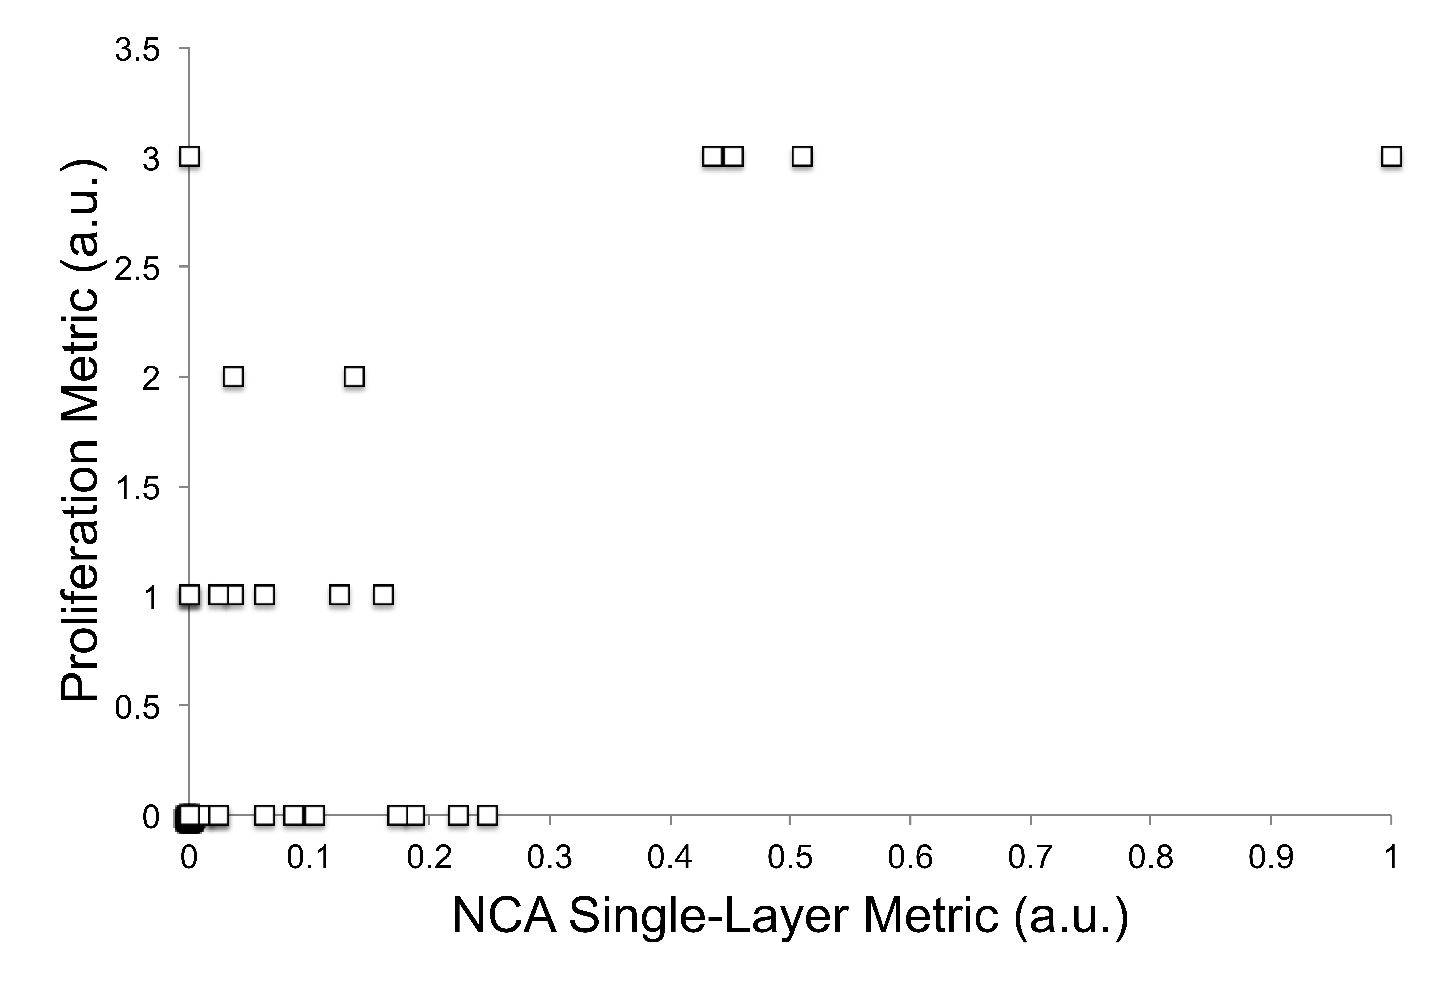
\includegraphics[width=0.7\textwidth]{nca_1963.eps}
  \caption{For the year 1963, the proliferation metric for each node is plotted against the normalized NCA single-layer network metric. Overlapping data points at the origin represent states that do not engage in NCAs and exhibit no nuclear weapons activity. The Pearson correlation coefficient, $w_{\text{NCA}}(1963)$, for these two variables is 0.77. A value of $w_x$=1 would correspond to a perfect positive linear relationship between the two variables.}
  \label{fig:snap2}
\end{figure}

Weighting factors are determined on a year-by-year basis as the correlation between the $\widehat{R_{i|x}(t)}$ values in a given layer and a proliferation metric, $p$, obtained using a linear scale derived from known historical cases of nuclear weapons inactivity ($p=0$), exploration ($p=1$), pursuit ($p=2$), and acquisition ($p=3$) (Singh 2004). This is illustrated in Figure~\ref{fig:snap2} for all nodes using the NCA single-layer network metric in the year 1963. The weighting factor, $w_x$, is quantified using the Pearson correlation coefficient between the proliferation metric and the single-layer network metrics (Pearson 1929; Pearson 1931; Edgell and Noon 1984). Let $k$ be the total number of nodes in the network (k=78 for this study due to data availability). Then, $w_x$ is calculated on a year-by-year basis using the variances and covariances of the proliferation metric, $p$, and the single-layer metric $R_{i|x}$:
\begin{center}
\begin{equation}
\begin{aligned}
w_x = \dfrac { \sum_{i=1}^k(p_i - \bar{p})(R_{i|x} - \overline{R_{x}})} {\sqrt{\sum_{i=1}^k(p_i - \bar{p})^{2}}  \sqrt{\sum_{i=1}^k(R_{i|x} - \overline{R_{x}})^{2}}},
\end{aligned}
\end{equation}
\end{center}
where $p_i$ is the proliferation metric of the $i$th node in a given year, $\bar{p}$ is the mean of the proliferation metrics for all nodes in a given year, $R_{i|x}$ is the single-layer metric of the $i$th node in a given year, and $\overline{R_{x}}$ is the mean of the single-layer metrics for all nodes in the $x$th layer in a given year. 

\begin{figure}
  \centering
  \includegraphics[width=0.77\textwidth]{fourpanel-color.eps}
  \caption{The weighting factors for the threat, alliance, trade and NCA network layers as a function of year. The annual weighting factor is obtained as the Pearson correlation coefficient between the single-layer metrics and the proliferation metric for all states in a given year.}
  \label{fig:alliance_weights}
\end{figure}

The weighting factors for the NCA, threat, alliance, and trade layers as a function of year are shown in Figure~\ref{fig:alliance_weights}. A number of observations can be made from an examination of the correlations between these various international relations and proliferation status. The NCA metric consistently has the highest correlation with proliferation-relevant activity since 1955, whereas the correlation between alliances and proliferation-relevant activity steadily and consistently decreases as a function of time. The correlation values for trade are negative, which may speak to the power of a highly interconnected global economy to dissuade states from engaging in taboo behaviors that would result in isolation and economic sanctions. The correlation between threat and nuclear proliferation has varied throughout the nuclear age, suggesting that states may have more or less tolerance for the threat environment depending on the international context.  The authors believe that the influence of NCAs may have declined, though, in more recent years than those covered by the study, as knowledge of nuclear science and engineering has grown and spread.

\subsection{Results and Discussion}

The robustness of this network model of external nuclear proliferation determinants is evaluated using both a statistical analysis over the year range of 1951-1992\footnote{As layer weights are determined from data in the previous year, the start year for analysis (1951) is one year past the start year for collection of historical data (1950).} and an examination of a variety of case studies. Even with a ``perfect" description of a system and its interactions, the accuracy of the model output will be dependent upon the accuracy of the input parameters; this analysis is limited by the inevitable incompleteness of the historical record. Further, uncertainty in the model input due to both lack of knowledge (e.g., an undocumented NCA) and inherent variability (e.g., ordinal coding of the threat of force in conflict intensity using qualitative and somewhat subjective metrics) results in uncertainty on the resultant SPMs. In lieu of a probabilistic uncertainty assessment of model inputs, a statistical analysis is performed here to quantify the impact of input data uncertainty on model performance.  


\subsection{Statistical Analysis}

\begin{table}
\centering
\caption{Average Ordinal Rank of Proliferation Transitions \label{tab:trans}}
\begin{tabular}{l|ccc}
\hline\noalign{\smallskip}
 & \multicolumn{3}{c}{Transition Type}\\
  & 2 $\rightarrow$ 3 & 1 $\rightarrow$ 2  & 0 $\rightarrow$ 1 \\
\noalign{\smallskip}
\hline
\noalign{\smallskip}
This model & 12.9 $\pm$ 10.8 & 18.5 $\pm$ 16.9 & 32.1 $\pm$ 23.3\\
Uniform Random Distribution & 36.8 $\pm$ 7.5 & 36.7 $\pm$ 6.3 & 37.3  $\pm$ 5.5\\
Extreme Value Random Distribution & 36.9 $\pm$ 7.5 & 36.7 $\pm$ 6.3 & 37.2 $\pm$ 5.5 \\
\hline
\end{tabular} 
\end{table}

To explore the functionality of this network model from an overarching perspective, the ordinal rank of a state in the SPM distribution (ordered from high to low for the 78 states considered in this study) was calculated in the year the state underwent a transition in proliferation stage. The proliferation stage is quantified using the proliferation metric, $p$, described in Section~\ref{rep}. States having already achieved nuclear weapons acquisition were excluded from the ranking. The ordinal ranks were then averaged for all states in the year range of 1951-1992 undergoing 2 $\rightarrow$ 3 (pursue to acquire), 1 $\rightarrow$ 2 (explore to pursue), and 0 $\rightarrow$ 1 (none to explore) transitions, respectively, as shown in Table~\ref{tab:trans}. The average rank of a state's SPM value decreases with increasing proliferation stage transition type, where a higher SPM value corresponds to a lower ordinal rank. That is, a state is more likely to have a higher SPM value when transitioning to a higher proliferation stage. The large standard deviations of the average ordinal ranks for all transition types may be illustrative of the degree to which external factors alone were globally relevant as proliferation determinants during this period. In addition, the small sample size may influence variability. 

To evaluate the statistical significance of these results, SPM values were randomly sampled with 10,000 trials from uniform and generalized extreme value (Coles 2001) distributions, and an average ordinal rank and standard deviation were calculated. A generalized extreme value distribution was chosen as it best mimicked the tail behavior of the SPM distribution at high SPM values. As shown in Table~\ref{tab:trans}, the average ordinal rank and standard deviation of the synthetic data is largely independent of the shape of the random variable distribution. Even with the large variance on the model output, the ordinal rank for 2 $\rightarrow$ 3 transitions is lower than that for the random distributions within one standard deviation. 

\begin{figure}
  \centering
  \includegraphics[width=0.74\textwidth]{TopTen-color.eps}
  \caption{Histogram of the number of occurrences in the top ten ranking of the SPM by state. The number in parentheses following the state name is the maximum value of the proliferation stage metric achieved by that state over the year range of 1951-1992. Striped orange bars indicate Latin American states, shaded blue bars indicate states covered by the U.S. nuclear umbrella, and crosshatched green bars indicate other notable cases.}
  \label{fig:topten}
\end{figure}

A histogram of the number of occurrences of a state in the top ten SPM ranking over the year range of 1951-1992 for the twenty  states that appear in the top ten most frequently, excluding nuclear weapons states, is shown in Figure~\ref{fig:topten}. The maximum value of the proliferation stage metric for the state over this same time period is denoted in parentheses following the state name. The results largely fall into two main categories: (1) states covered by the U.S. nuclear umbrella and (2) Latin American states. Other notable cases include North Korea, Iraq, Iran, and Jordan.

Canada, Netherlands, Italy, Belgium, Spain, Japan, South Korea, and Sweden\footnote{Though not a member of NATO, Sweden was extended \textit{de facto} U.S. nuclear umbrella coverage through NSC 6006/1 (Tertrais 2011).} are all covered under the U.S. nuclear umbrella through the North Atlantic Treaty Organization (NATO) or other agreements, with several of these states being host to U.S. tactical nuclear weapons. While U.S. alliance commitments to these countries were represented in the model, there was no distinction for nuclear umbrellas, which may have been a key factor in why these states--which had both nuclear capabilities and threat motivations--did not proliferate. On the other hand, Latin American states represent a different geopolitical dynamic. They are in a region with no nuclear-armed adversaries and many have commitments to, or may be influenced by, the Treaty of Tlatelolco (Treaty for the Prohibition of Nuclear Weapons in Latin America and the Caribbean), which formed the basis for a Nuclear Weapons Free Zone (NWFZ) in Latin America (Goldblat 2004). The Latin American states' (and Jordan's) SPM values are largely driven by threat and alliances, but they lacked the foundational nuclear capabilities to proliferate. Notable exceptions are Brazil and Argentina (explored in further detail in Section~\ref{Arg-and-Braz}), which used NCAs to establish a capability to reach the ``pursue" stage of proliferation. Finally, North Korea, Iraq, and Iran may illustrate the limits of a model that considers only external factors, given that these states were relatively isolated from the international economy and developed their nuclear weapons programs without much official external assistance. 

A histogram of the number of occurrences of a state in the bottom ten ranking in the SPM distribution over the year range of 1951-1992 yielded similarly consistent results. Any state that occurred more than ten times in the bottom ten of the distribution either never pursued a nuclear weapons program (i.e., Albania, Luxembourg, Mongolia, Ethiopia, New Zealand, Nepal, Indonesia, Myanmar, Liberia, Sri Lanka, Austria, Finland, and Ireland) or had, at maximum, a period of nuclear weapons exploration (i.e., Sweden and Australia).   

\subsection{Case Studies}

Case studies include South Africa, North Korea, and two case pairings for comparative purposes: Argentina and Brazil, and India and Pakistan. South Africa's unique history as the only nuclear-armed state to voluntarily give up nuclear weapons impelled its inclusion. North Korea, with its spate of internal factors not represented in the model, was included to examine the degree to which the model performs in an internally-dominated scenario. The regional dynamics of Argentina/Brazil and India/Pakistan, coupled with proliferation-motivating rivalry left unquantified in the model, create powerful comparative examples. 

\subsection*{South Africa}

The SPM of South Africa, as shown in Figure~\ref{fig:southafrica}, demonstrates that the state's primary external proliferation motivation was threat. South Africa's nuclear weapons pursuit began in 1974, coinciding with increasing security threats in the region, primarily from Cuba and the Warsaw Pact states encroaching upon South African borders (Stumpf 1995). While South Africa's NCAs did contribute to an overall higher SPM, the acquisition of NCAs does not align with actual proliferation timelines. Nuclear latency, defined as the possession of the technologies, facilities, materials, expertise, and other capabilities required for nuclear weapons development \textit{without} the development of a nuclear device, may have resulted in a time lag between nuclear weapons technology acquisition and increasing proliferation stage. South Africa's proliferation timeline (i.e., the proliferation stage metric in Figure~\ref{fig:southafrica}) closely mirrors the increasing threat. The state's nuclear latency, driven in part by NCA contributions up to the early 1970s, set the stage for proliferation in step with a rising tide of conflict.  

\begin{figure}
  \centering
  \includegraphics[width=0.77\textwidth]{SouthAfrica.eps}
  \caption{The SPM for South Africa as a function of year. The single-layer contributions to the SPM are shown in the stacked bar and the total SPM is given by the filled diamonds. South Africa's proliferation stage is plotted on the secondary ordinate axis. The total SPM is lower than the sum of each single-layer contribution as trade accounts for a negative impact on SPM values.}
  \label{fig:southafrica}
\end{figure}

\subsection*{North Korea}

\begin{figure}
  \centering
  \includegraphics[width=0.77\textwidth]{NorthKorea.eps}
  \caption{The SPM for North Korea as a function of year. The single-layer contributions to the SPM are shown in the stacked bar and the total SPM is given by the filled diamonds. North Korea's proliferation stage is plotted on the secondary ordinate axis.}
  \label{fig:nk}
\end{figure}

As shown in Figure~\ref{fig:nk}, North Korea's SPM does not exhibit a consistent trend as a function of time. Lack of trade, a negative proliferation correlate, leads to total SPM values that are generally higher in magnitude than would be expected for a non-isolated state. The total SPM values are largely dominated by contributions from the threat layer, driven by continued conflict with the United States and South Korea. The somewhat erratic trend in the data as a function of time is due to the constant flux in the three states' posturing and military capability; additionally, the spike in the mid-1980s could be an artifact of the higher threat correlation coefficient in the previous year.

There is no clear correlation between the SPM data and North Korea's proliferation timeline. It could be argued that North Korea's proliferation motivation was largely driven by internal determinants not considered in this model. North Korea is an authoritarian regime with the power to put military might and prestige above other typical state concerns (Hymans 2008). By cutting themselves off from the world with incendiary rhetoric and flaunting of Nuclear Non-Proliferation Treaty (NPT) obligations, the North Korean leadership demonstrated that they are a different type of government not highly influenced by international nonproliferation norms. As internal determinants are not included in this model, the ``rogue state" case fails to yield meaningful results.


\subsection*{Argentina and Brazil}
\label{Arg-and-Braz}

Argentina and Brazil represent a complex case of regional power rivalry driven in part by domestic politics. Both states undertook mutual efforts to obtain nuclear weapons and began nuclear weapons pursuit contemporaneously in 1978. However, while Argentina's SPM value (shown in Figure~\ref{fig:arg}) trends well with its proliferation metric, the SPM for Brazil (shown in Figure~\ref{fig:braz}) is not well correlated with its proliferation timeline. The total SPM for Argentina tends to increase with time driven largely by increasing contributions from the threat and NCA single-layer network metrics. In contrast, the SPM for Brazil peaks in 1968 and exhibits a roughly decreasing trend in the following years led by the decreasing alliance single-layer network metric. 

\begin{figure}
  \centering
  \includegraphics[width=0.77\textwidth]{Argentina.eps}
  \caption{The SPM for Argentina as a function of year. The single-layer contributions to the SPM are shown in the stacked bar and the total SPM is given by the filled diamonds. Argentina's proliferation stage is plotted on the secondary ordinate axis.}
  \label{fig:arg}
\end{figure}

\begin{figure}
  \centering
  \includegraphics[width=0.77\textwidth]{Brazil.eps}
  \caption{The SPM for Brazil as a function of year. The single-layer contributions to the SPM are shown in the stacked bar and the total SPM is given by the filled diamonds. Brazil's proliferation stage is plotted on the secondary ordinate axis.}
  \label{fig:braz}
\end{figure}

Internal politics may have been a strong proliferation influence for both states and is not reflected in the model. Brazil endured a 1964 government takeover by its military and the eventual return of a civilian government in 1985. Similarly, in 1976, the Argentina military established a junta government through a successful coup attempt just prior to the state's transition to nuclear weapons pursuit (Cirincione et al. 2005, 384). The lack of militarized disputes and muted hostility between the two states precludes the incorporation of their rivalry dynamic in the threat metric. This may contribute in some part to the inability of the model to capture Brazil's proliferation timeline, whereas Argentina's history of conflict with Chile and, later, the United Kingdom is manifest in the threat single-layer network metric. Nonetheless, it is largely Argentina's increasing NCA single-layer network metric that best trends with its escalating nuclear weapons program. 

\subsection*{India and Pakistan}

India and Pakistan are classic examples of threat-driven proliferation enabled by foundational nuclear capabilities established through NCAs and the Atoms for Peace program. In both cases, the decision to pursue nuclear weapons has often been attributed to the desire to obtain a ``trump card" or equalizer. Although often intertwined, India's proliferation was much less driven by Pakistan than vice versa (Reed and Stillman 2010).  

India was one of the first states to participate in and benefit from the Atoms for Peace program. Its first reactor came on-line in 1956, less than three years after Eisenhower's speech announcing the program (ACDIS 2016). Prior to the NPT entry into force in 1970, India continued to sign many NCAs establishing a strong baseline nuclear capability. This is reflected by the NCA single-layer metric comprising a bulk of the SPM shown in Figure~\ref{fig:india}, which, on average, ranks 11$^{th}$ in the world between 1963-1992. However, India's progression from one proliferation stage to another is better indicated by the threat data. For example, the decision to move to nuclear weapons pursuit in 1964 was preceded by the Sino-Indian War of 1962 and  roughly coincident with the first Chinese nuclear weapons test of 1964. Furthermore, the decision to deprioritize its weapons program with a return to exploration in the late 1970s after the demonstration of a ``peaceful nuclear explosion" coincided with a lull in external threats as shown in Figure~\ref{fig:india} and resumption of diplomatic ties with China in 1976 (Gopalan 1992, 1401--1402). The decision to acquire the bomb in 1988 coincides directly with the announcement of Pakistan's nuclear bomb by AQ Khan in 1987 and the Sino-Indian skirmish of the same year.  

\begin{figure}
  \centering
  \includegraphics[width=0.8\textwidth]{India.eps}
  \caption{The SPM for India as a function of year. The single-layer contributions to the SPM are shown in the stacked bar and the total SPM is given by the filled diamonds. India's proliferation stage is plotted on the secondary ordinate axis.}
  \label{fig:india}
\end{figure}

\begin{figure}
  \centering
  \includegraphics[width=0.8\textwidth]{Pakistan.eps}
  \caption{The SPM for Pakistan as a function of year. The single-layer contributions to the SPM are shown in the stacked bar and the total SPM is given by the filled diamonds. Pakistan's proliferation stage is plotted on the secondary ordinate axis.}
  \label{fig:pakistan}
\end{figure}

Like India, Pakistan benefited from NCAs and the Atoms for Peace program, but its first reactor did not come on-line until 1972. Unlike India, whose SPM rose with increasing capability, Pakistan's SPM remained roughly constant from the mid-1950s to the early 1990s as shown in Figure~\ref{fig:pakistan}. This could explain the jump over the ``explore" stage directly to pursuit in 1972 upon establishment of nuclear capabilities through NCAs. The SPM for Pakistan ranked 22$^{nd}$ in the world from 1965-1971, the period immediately preceding its decision to pursue a nuclear weapons program. This finding of a slightly above average SPM is consistent with Singh and Way's analysis indicating that Pakistan was an ``unlikely proliferator," where its external environment and nuclear capabilities did not illuminate its proliferation motivations (Singh and Way 2004, 880). According to the model, Pakistan's decision to advance to the ``acquire" proliferation stage could be partially motivated by the Siachen Conflict with India that took place over the late 1980s.

While the SPM and single-layer network metrics can be used to explain a significant portion of both India and Pakistan's decisions to proliferate, it does not capture the full story in either case. India maintained a constant SPM in the late 1970s when it decided to return to exploration following its nuclear test. Additionally, its decision to move to nuclear weapons pursuit in the 1980s cannot be explained in terms of its SPM, but is likely due to the rise of the Pakistani nuclear weapons program, a rivalry fueled by security threats posed by non-state proxies and not captured in the threat single-layer network metric. Pakistan's SPM is consistently among the lowest values recorded for Pakistan during the time that Pakistan jumped to nuclear weapons pursuit in the early and mid-1970s. Finally, although partially motivated by threat, the largest contributor to the timing of Pakistan's acquisition of a nuclear weapon may be latency due to delays in technology maturation. 


\subsection{Model summary}

This network model allows for a quantitative investigation of the impact of various external factors on proliferation motivation. This work may illuminate subtle and nascent proliferation risks, and provides a framework for policymakers to consider the proliferation effects of new alliances, threats, NCAs, and trade agreements. The model can be refined in resolution, e.g., inclusion of regional rivalry data, strategic trade, nonproliferation and NWFZ treaties, nuclear umbrella coverage, \&c., with different intra- and inter-layer network dynamics, and presents varied opportunities for further research. 

The model results trend well with historical data for states whose primary proliferation motivators are external. Expanding the node attributes for each state may allow for modeling internal determinants in addition to the external factors discussed herein. As the threat profile of a conflict is dependent in part on the relative military strengths of the adversaries, the value of alliances and trading relationships may vary depending on the ally and the trading partner, respectively. Though difficult to quantify, internal determinants such as regime type, economic policies, nonproliferation norms, and prestige motivations present potential proliferation correlates worth examination (Sagan 1996). 

Another prospective area of exploration is indirect ties, which have been shown to affect the security-seeking behavior of states (Gartzke et al. 2014, 500--502). Recent research demonstrates that mutual membership in an informal trading community decreases the likelihood of conflict between two states, even if they do not directly trade in high volumes (Lupu and Traag 2012, 1033--1034). By altering the security-seeking behavior of member states, communities of traders, allies, and enemies may shape proliferation behavior.

Despite the strong correlation between proliferation and internal state factors, this multiplex network model \textit{considering only limited external relations} correlates with state proliferation timelines at a level consistent with other models with similar goals. This work represents the first quantitative heterogenous analysis of proliferation determinants using a network science formalism and moves the field forward in quantifying nuclear proliferation motivation, and in a broader sense, international relations. 

We expect to show the work described above to personnel at the State Department Arms Control, Verification, and Compliance office in concert with DNN sponsors.  

\newpage
\thispagestyle{empty}
\mbox{}
\newpage

\section{Publications}
\subsection{Invited Book Chapter: Societal Verification}
In April, co-PI Zoe Gastelum submitted (with some support from NetSci funding) an invited book chapter: Gastelum, Zoe N. `Societal Verification for Nuclear Nonproliferation and Arms Control,' for \textsc{Nuclear Non-proliferation and Arms Control Verification: Innovating Systems Concepts}, ed. Mona Dreicer, Irmgard Niemeyer, and Gotthard Stein. The chapter drew heavily on the new media sources described in the section above, and explored societal verification through two mechanisms of collecting and analyzing societally-produced data, \textit{viz.,} mobilization and observation. It described current applications and research in each area before providing an overview of challenges and considerations that must be addressed in order to bring societally-produced data into an official verification regime. The chapter concluded by emphasizing that the role of societal verification, if any, in nonproliferation and arms control will supplement, rather than supplant, traditional verification means.

\subsection{Conference and journal publications}
J. H. Kornell, Z.N. Gastelum, B.L. Goldblum, `Informational Sensing for Nonproliferation,' in Proceedings of the Advances in Nuclear Nonproliferation Technology and Policy Conference, Santa Fe, 2016 (American Nuclear Society, 2016) No. 18849.

N. Mahowald, B.L. Goldblum, T. Hickey, J.H. Kornell, `Quantifying Correlations between International Relations and Nuclear Proliferation Status,' in Proceedings of the Advances in Nuclear Nonproliferation Technology and Policy Conference, Santa Fe, 2016 (American Nuclear Society, 2016) No. 18857.

The model-centric material above is being written for submission to the Journal of Conflict Resolution. 

\pagebreak
\section*{Acknowledgements}

The multiplex network approach was suggested by Tracy Kuo Lin and Vikram Vijayaraghavan, recipients of the 2014 Network Science Idea Challenge Award. This material is based on work supported by the Department of Energy National Nuclear Security Administration through Award Number DE-AC52-06NA25048, and by the Department of Energy National Nuclear Security Administration through the Nuclear Science and Security Consortium under Award Numbers DE-NA-0000979 and DE-NA-0003180. The authors thank Oliver Matheau-Raven and James Delaney for assistance with methods and evaluation of analyses and computations, Rebecca Krentz-Wee for assistance in literature search for case study evaluations,  J.A. Brown for software development support. We were materially aided by UC Berkeley students and graduate students Thomas C. Hickey, James Bevins, Elie Katzenson, Sarah Laderman, Nathaniel Mahowald, Yara Mubarak, and David Sweeney.


\end{document}